\documentclass[12pt]{standalone}

% Sequence: [0,13,14,4,13,1,5,7]

\usepackage{tikz}

\begin{document}
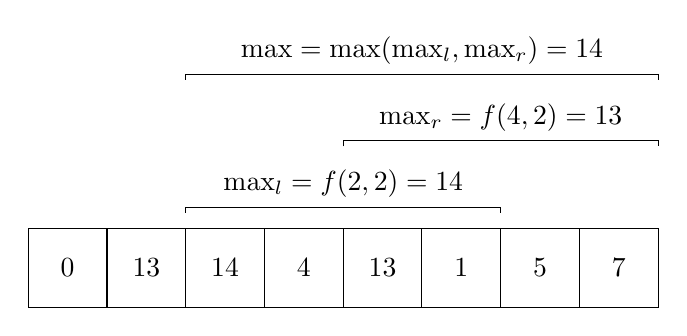
\begin{tikzpicture}[x=1cm,y=1cm]

\begin{scope}
    [every node/.style={draw,rectangle,minimum size=1cm},
        xshift=0.5cm,yshift=0.5cm]
    \node at (0,0) {$0$};
    \node at (1,0) {$13$};
    \node at (2,0) {$14$};
    \node at (3,0) {$4$};
    \node at (4,0) {$13$};
    \node at (5,0) {$1$};
    \node at (6,0) {$5$};
    \node at (7,0) {$7$};
\end{scope}

\begin{scope}[y=24pt,yshift=12mm]
    \draw (2,0) -- ++(0,2pt)
        -- node[above] {${\max}_l = f(2,2) = 14$} ++(4,0)
        -- ++(0,-2pt);
    \draw (4,1) -- ++(0,2pt)
        -- node[above] {${\max}_r = f(4,2) = 13$} ++(4,0)
        -- ++(0,-2pt);
    \draw (2,2) -- ++(0,2pt)
        -- node[above] {${\max} = \max(\max_l, \max_r) = 14$} ++(6,0)
        -- ++(0,-2pt);
\end{scope}


\end{tikzpicture}
\end{document}
